\documentclass[]{article}
\usepackage[margin=1in]{geometry}
\usepackage{hyperref}
\hypersetup{
	colorlinks=true,
	linkcolor=blue,
	filecolor=magenta,      
	urlcolor=blue,
}

\usepackage{graphicx}
\graphicspath{ {./images/} }
\usepackage{caption}
\captionsetup[figure]{labelformat=empty}
\usepackage{float}
\usepackage{wrapfig}
\usepackage{array}
\newcolumntype{P}[1]{>{\centering\arraybackslash}p{#1}}

%opening
\title{Secret Hitler AI}
\author{James Camacho}

\begin{document}

\maketitle

The goals of my project were twofold. First, I wanted to be able to detect which players were fascists, and second, I wanted to build an AI that could play Secret Hitler well.
\vspace{0.25cm}\newline
\emph{Part I. The Discriminator}
\newline\indent
Reading facial expressions or quavers in someone's voice is normally how a human would go about detecting if someone is lying, but that is pretty hard for a neural network to accomplish. Even humans aren't very good at it (only about 65\% accurate). Plus, there is a silent version of the game you can play on \href{secrethitler.io}{secrethitler.io} where all you see are the actions people take like voting, card claiming, etc. So I decided to only give actions as inputs.
\newline\indent
The model I chose for my neural network was a GRU with 3 hidden layers containing 100 neurons each. Then it had a linear layer that went to 21 outputs, 1 for each role each player in the game could be. These outputs were combined into 7 groups of 3 that were softmaxed to give the probabilities each player was either liberal, a regular fascist, or Hitler.
\newline\indent
To train my neural net I took an archive of games on \href{secrethitler.io}{secrethitler.io} (\href{http://secrethitler.io/public/gameDumps/gameSummaries.tar.gz}{download}), and cleaned it to be about 10,000 games which ended properly (no one quitted or got disconnected) and played by the normal seven-player rules. Then I changed the game logs into one-hot (well, several-hot) vectors representing different actions. I used cross entropy loss after every turn on the outputs.
\newline\indent
The results were not very impressive. The loss did go down, and the loss at the end of the game was less than at the beginning.
However the decrease in loss was not very significant. Furthermore, the accuracy—determined by which players the neural net thought was most fascist—never improved, it was always the same throughout the entire game and just jumped around 43\% accuracy throughout training (which is what it would get by pure guessing).
\begin{figure}[H]
\centering
\begin{minipage}{0.5\textwidth}
	\centering
	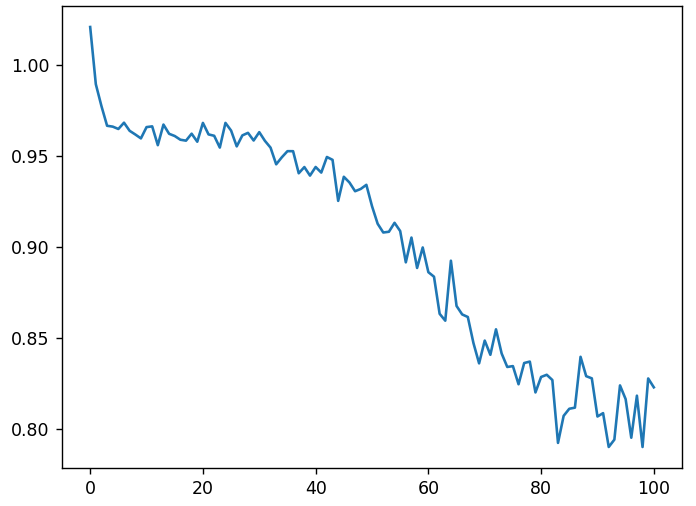
\includegraphics[width=0.9\textwidth]{loss}
	\caption{Losses}
\end{minipage}\hfill
\begin{minipage}{0.5\textwidth}
	\centering
	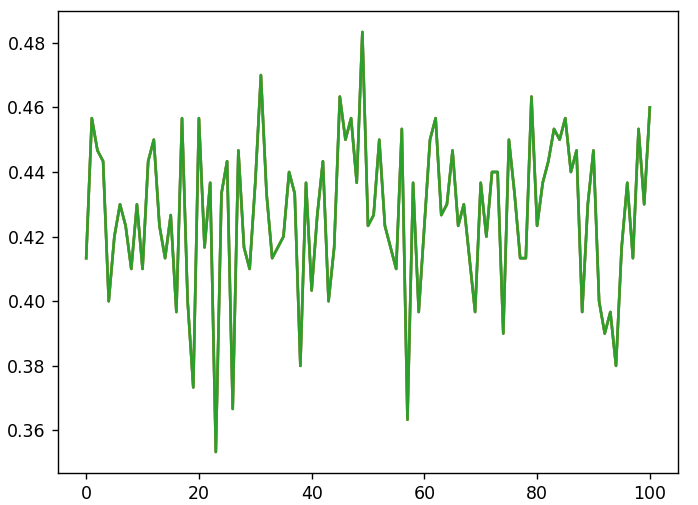
\includegraphics[width=0.9\textwidth]{accuracies}
	\caption{Accuracies}
\end{minipage}
\end{figure}
This suggests that the neural net just regressed to the mean. Adding more hidden layers or neurons did not improve the network's performance. My best guess is the inputs fed into the network were hard for it to use.
\vspace{0.25cm}\newline\noindent
\emph{Part II. Playing the Game}
\newline\indent
I used self-play combined with reinforcement learning to make an AI to play the game intelligently. Originally I was going to use a \emph{predictor} to begin the self-play, which would be similar to the discriminator except that instead of outputting suspected roles it would output next moves. However, after the discriminator failed to work, I decided that it wouldn't be any worse to start out using (partly) random bots. They would vote, pick, investigate, discard, and claim randomly, except a few special cases; fascists wouldn't shoot Hitler, and liberals wouldn't discard liberal cards or claim incorrectly.
\newline\indent
My AI player uses a qtable to determine the best moves to play. Of course, the qtable was approximated by a neural net: a GRU with 5 layers and a hidden size of 300, and one linear layer that ended in a tanh to give the computed q-value. The AI would consult it's qtable on the various actions it could take and then play what it thought was the best move. Picking cards turned out to be trickier though, because the AI as President had no way of knowing what the Chancellor would do, and as Chancellor didn't know what the President would claim they did. I attempted to have it try one (or all, and choose the minimum q-value) of the possibilities that could happen, but it didn't seem to improve the AI, so I scrapped that idea. Instead, the AI just always chose liberal cards as liberal and fascist cards as fascist.
\newline\indent
Training involved playing against the random bots. A win was given a reward of 1, and a loss a reward of -1. Anything else was a reward of 0. After one AI was trained for 500 games it would be entered into the pool of players that new AI's would train against. The AI's weren't exceptionally good, but they were better than the random bots.
\newline\indent
You can see that the first AI which trained against only random bots has a higher winrate than them all, and the second AI which also trained against the first one has an even higher winrate. Eventually I implemented a simple elo system. Here are six trained AI's; the bottom elo is from a random player.
\newline
\begin{figure}[H]
	\centering
	\begin{minipage}{0.5\textwidth}
		\centering
		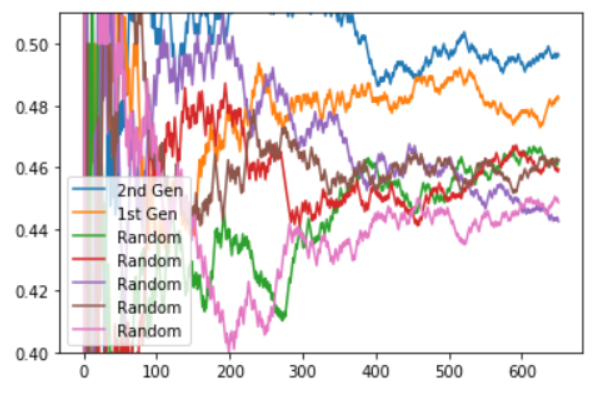
\includegraphics[width=0.9\textwidth]{twogens}
		\caption{Win Rates}
	\end{minipage}\hfill
	\begin{minipage}{0.5\textwidth}
		\centering
		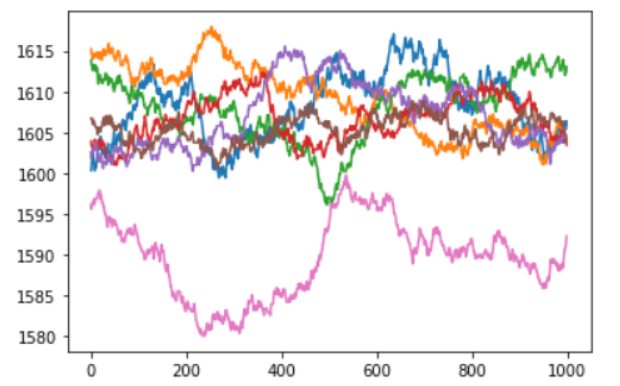
\includegraphics[width=0.9\textwidth]{manygens}
		\caption{Elos}
	\end{minipage}
\end{figure}
\begin{wrapfigure}{r}{0.4\textwidth}
	\centering
	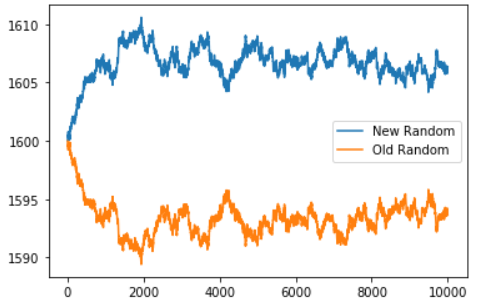
\includegraphics[width=0.4\textwidth]{tworandoms}
	\caption{Elos}
\end{wrapfigure}
The trained AI's clearly do better than the random players, but that could just be from how they pick cards. After all, the fascist random players could be picking liberals and helping their opposition. I ran 10,000 matches between random players that picked cards randomly, and ones that picked cards like the AI's did. The results showed that it \emph{did} give them a significant advantage. However, the graph of the win rates suggests that the AI's were learning something, and not just given an advantage to begin with. Also, the when the elo of one AI started going up so did the elos of the other AI's, which suggests they were learning some kind of meta and working together.
\newpage
\noindent
\centerline{\textbf{Time Log}}
\renewcommand{\arraystretch}{2}
\begin{table}[H]
	\begin{tabular}{|P{0.1\textwidth}|P{0.15\textwidth}|p{0.75\textwidth}|}
		\cline{1-3}
		Date    & Time Spent (minutes) & Tasks                                                                                                                                                                                                                                                                                                \\ \cline{1-3}
		3/20/21 & 165                  & Obtaining and cleaning data, began building the discriminator.                                                                                                                                                   
		\\ \cline{1-3}
		3/22/21 & 180                  & Changed inputs to not include every action, mostly finished discriminator module and started training and testing it.   
		\\ \cline{1-3}
		4/8/21  & 120                  & Added batching to the discriminator, reverted back to full input data, and made graphs.  
		\\ \cline{1-3}
		4/9/21  & 135                  & Built random player, started work on game interface for bots to play with.    
		\\ \cline{1-3}
		4/10/21 & 180                  & Finished game interface and the AI class. Got one to train.                                                                                                                                                       
		\\ \cline{1-3}
		4/12/21 & 120                  & Tried using the qtable to pick cards, working on self-play (not just against random players).             
		\\ \cline{1-3}
		4/14/21 & 120                  & Implemented elo system, removed the different way of picking cards (didn't work better). Mostly finished self-play.        
		\\ \cline{1-3}
		4/15/21 & 90                   & Analyzing results and testing different things now. Tried using a smaller neural net to approximate the qtable and it worked about as well.             
		\\ \cline{1-3}
		4/16/21 & 240                  & The AI seems to be nearly picking randomly because of how close the q-values always are. Switched the structure of the neural net to (hopefully) make them less similar, and also how the AI uses the qtable to determine moves. Also changed the random player so it picked cards a little smarter. 
		\\ \cline{1-3}
		4/17/21 & 180                  & Try regular recurrent network as opposed to GRU with the discriminator, testing the better random player against the dumber one, and writing up this report.          \\ \cline{1-3}                                                                                                               
	\end{tabular}
\end{table}
\textbf{Total Time (hours):} 25.5

\newpage
\noindent
\textbf{Addendum: A Brief Explanation of Secret Hitler}
\newline\indent
Secret Hitler is a social deception game. Two teams—the fascists and the liberals—attempt to enact their own policies on the board. The liberals have four players on their team and will win if they can enact five liberal policies, while the fascists have only three players and need to enact six fascist policies to win. However, the fascists have a few advantages: there are seventeen fascist policies in the deck as opposed to only six liberal ones, the fascists (with the exception of Hitler) know who each other are, and the fascists have an alternate win condition by electing Hitler as chancellor after three fascist policies have already been enacted.
\newline\indent
Each player takes turns being the President. On their turn, they pick a Chancellor, and if a majority of the players approve the cabinet, the President and the Chancellor get to enact a policy. The President draws three cards from the top of the deck, and chooses one \emph{without showing anyone else} to discard. The Chancellor does the same with the remaining two cards, leaving one policy to be enacted. If a liberal policy is played, everyone cheers, while if a fascist policy is played the President gets one of three powers depending on how late in the game it is: investigation (seeing someone's role), special election (disrupting the turn order and choosing the next President), or kill power (eliminating someone from the game).
\newline\indent
The President and the Chancellor can lie about anything in the game. For example, if a fascist President draws two fascist policies and one liberal one, they could discard the liberal one and claim to have gotten three fascist policies (i.e. so they were "forced" to enact a fascist policy even though they "didn't" want to). It is practically never advantageous for a liberal to lie, and in fact \href{secrethitler.io}{secrethitler.io} has a rule against lying as a liberal.
\vspace{0.5cm}
\newline

\end{document}
